\section{Fallstudien}\label{sec:fallstudien}

Die aggregierten Kennzahlen liefern einen guten Überblick über die Modellqualität, verbergen jedoch individuelle Fehlklassifikationen. Im Folgenden verdeuttlichen drei ausgewählte Fallstudien typische Muster von \ac{FP} und \ac{FN}.

\subsection*{Sales Warehouse}

Der englische Prozess \enquote{Sales Warehouse} aus dem Datensatz \enquote{Universität} enthält vier als kritisch gelabelte Aktivitäten und ist in Abbildung \ref{fig:qwen3-fall} zu sehen. Das Modell \texttt{Qwen3-235B-A22B-Thinking-\linebreak~2507} klassifiziert die gelabelten korrekt, markiert jedoch zusätzlich die Aktivität \enquote{Ship product} als kritisch, was in \Abbildung{fig:qwen3-fall} als rot markierte Aktivität dargestellt ist. Die Begründung verweist auf die Nutzung der Kundenadresse für Versand und Zustellung. Obwohl während der Modellierung nur ein rein logistischer Schritt vorgesehen war - der laut Tabelle \ref{tab:labeling-examples} in dem Labeling-Guide nicht kritisch ist - interpretiert das Modell den möglichen Datenfluss und wählt eine konservative Einstufung. Angesichts des Zielkriteriums eines hohen Recalls ist dieses \ac{FP} vertretbar.

\begin{figure}
    \centering
    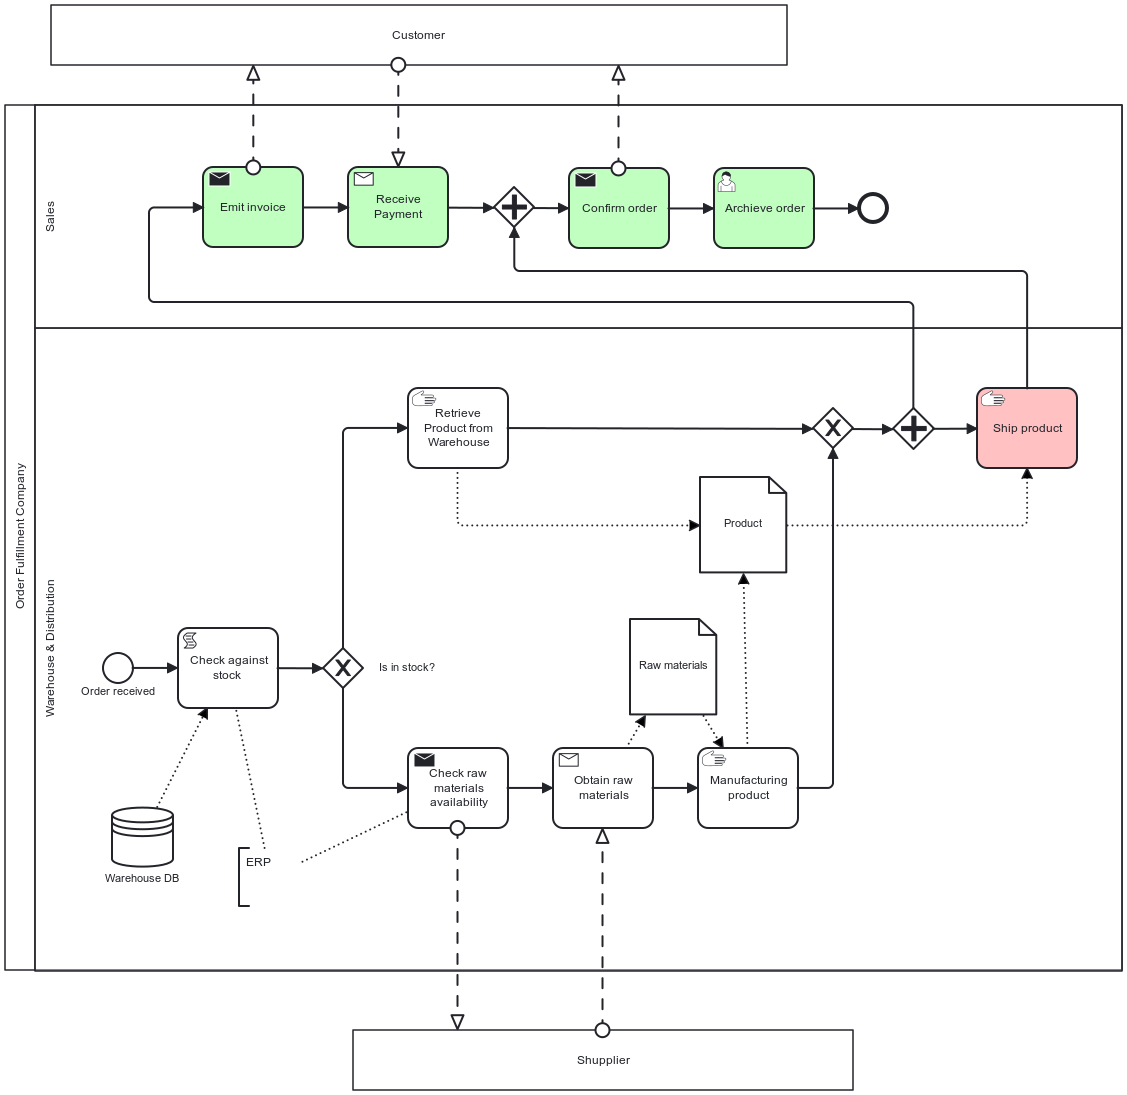
\includegraphics[height=.41\textheight]{images/results/examples/qwen3-235B-run-3-uni-sales-warehouse}
    \caption{Ergebnis des Testfalls \enquote{Sales Warehouse} mit farblich hervorgehobenen Aktivitäten. Grün markierte Aktivitäten sind korrekt als kritisch erkannt, rot markierte stellen \acp{FP} dar.}
    \label{fig:qwen3-fall}
\end{figure}

Das Beispiel verdeutlicht eine grundsätzliche Limitierung der Klassifizierung. Wenn in einem \ac{BPMN}-Modell explizite Informationen über Datenverarbeitungen fehlen, ist es für das das \ac{LLM} schwierig, eine eindeutige Klassifikation vorzunehmen.

\subsection*{Marketing-Kampagne}

Im deutschen Testfall \enquote{Marketing-Kampagne}, aus dem Datensatz \enquote{Kleine Szenarien}, sind drei Aktivitäten als kritisch gelabelt: \enquote{Leads sammeln}, \enquote{Newsletter versenden} und \enquote{CRM aktualisieren}. \texttt{GPT-OSS-20B} identifiziert diese korrekt, markiert aber zusätzlich die Aktivität \enquote{Klickraten auswerten} als kritisch. Im Prozessmodell wird davon ausgegangen, dass die Klickdaten vollständig anonymisiert werden, jedoch ist diese Information nicht explizit hinterlegt. Mehrere Modelle – darunter \texttt{Qwen3-235B-A22B-Thinking-2507} – stufen diesen Schritt daher als potenziell personenbezogen ein, wie in Abbildung \ref{fig:gptoss-fall} zu sehen ist. Die Anonymisierung der Daten wurde nur von \texttt{Mistral-7B-Instruct-v0.3} in zwei von fünf und von den Gemma-Modellen in allen Wiederholungen korrekt antizipiert und die Aktivität als unkritisch klassifiziert. Dieses Beispiel zeigt, wie fehlende Kontextinformationen zu vorsichtiger Klassifikation und damit zu \ac{FP} führen können.

\begin{figure}
    \centering
    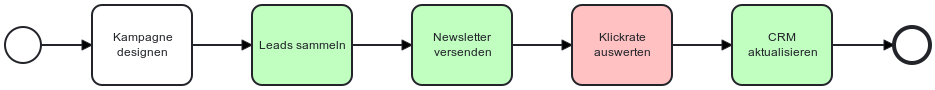
\includegraphics[width=\textwidth]{images/results/examples/oss-20b-run-1-small-marketing}
    \caption{Ergebnis des Testfalls \enquote{Marketing-Kampagne} mit farblich hervorgehobenen Aktivitäten. Die Aktivität \enquote{Klickraten auswerten} wurde als zusätzliches kritisches Element markiert.}
    \label{fig:gptoss-fall}
\end{figure}

Dieses Beispiel zeigt, dass ohne genaue Kontextangaben zur Anonymisierung selbst scheinbar unbedenkliche Auswertungen als datenschutzrelevant erscheinen können. Es unterstreicht, dass die \acp{LLM} im Zweifel eher ein kritisches Label vergeben, um \acp{FN} zu vermeiden, wie es das Hauptziel der Klassifikation aus Abschnitt \ref{sec:qualitatsziele} vorsieht.

\subsection*{Karten-App – Standort erfassen}

Der Testfall \enquote{Karten-App – Standort erfassen} besteht aus zwei Aktivitäten: \enquote{Standort erfassen} und \enquote{Route berechnen}. Beide sollten als kritisch klassifiziert werden, da im zweiten Schritt der erfasste Standort zur Berechnung der Route genutzt wird. \texttt{Mistral-Large-Instruct-2411} kennzeichnet jedoch in drei von fünf Wiederholungen nur die erste Aktivität als kritisch, wie in Abbildung \autoref{fig:mistral-fall} zu sehen. In der Begründung wird zwar die Verarbeitung personenbezogener Daten beim Erfassen des Standorts erkannt, dieser Zusammenhang aber nicht auf die nachfolgende Aktivität übertragen. Dieses \ac{FN} steht dem angestrebten hohen Recall entgegen und zeigt, dass einige Modelle Schwierigkeiten haben, Datenflüsse über mehrere Schritte hinweg zu verfolgen.

\begin{figure}
    \centering
    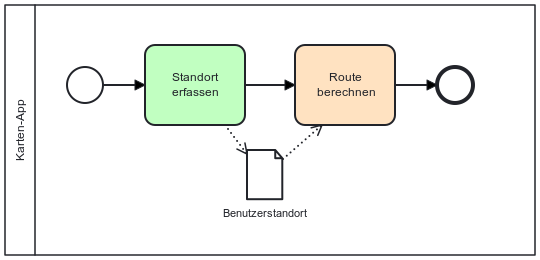
\includegraphics[width=.55\textwidth]{images/results/examples/mistral-large-run-3-small-maps-app}
    \caption{Ergebnis des Testfalls \enquote{Karten-App – Standort Erfassen} mit farblich hervorgehobenen Aktivitäten. Die Aktivität \enquote{Route berechnen} wurde fälschlicherweise nicht als kritisch markiert.}
    \label{fig:mistral-fall}
\end{figure}

Auf Basis der Erkenntnisse dieses gesamten Kapitels werden im folgenden Abschnitt die formulierten Forschungsfragen beantwortet. Dabei wird untersucht welches Modell sich insgesamt am besten für die Identifikation \ac{DSGVO}‑kritischer Aktivitäten eignet.